\section{Scalability} \label{section:scalability}
\large \textbf{Apache Kafka}\\
\normalsize
\textbf{Scalability of storage and computing server}\\
A Kafka broker serves read/write requests from clients as well as persisting the records on its disk. Therefore, the storage and processing layers are closely related and cannot be scaled independently.  

Topic partition is the basis element to achieve scalability on Kafka. Each partition can have one or more replicas, namely, a leader and a number followers for fault-tolerance. Each replica of a partition resides completely on the disk of a broker in the cluster. Read and write requests from client can only be done on the leader of a partition. Therefore, by distributing the leaders of partitions evenly among the brokers, the load on the serving layer can be balanced. Moreover, for each partition, to have even distribution, a different subset of brokers is selected to keep its replicas on their disks. A new broker can always be added to the cluster to scale up the capacity of both processing and persisting. When new partitions are created, their replicas will be automatically assigned to the new broker for load balancing.
\begin{figure}[h]
	\centering
	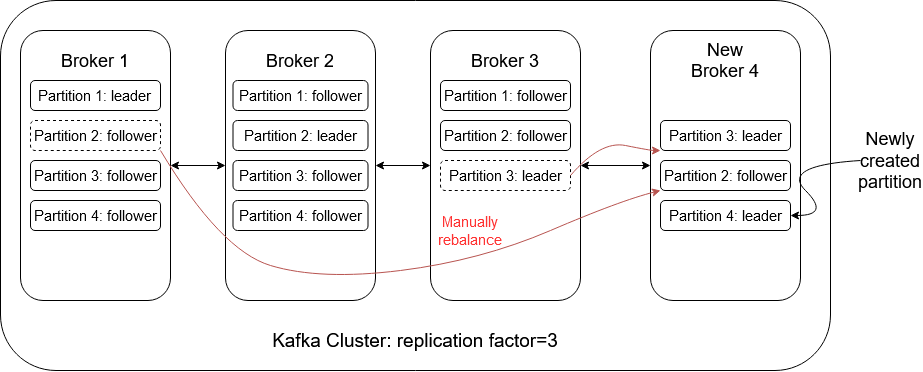
\includegraphics[width=\linewidth]{images/scalability-kafka.png}
	\caption{Kafka clustered is scaled up with a new broker.}
	\label{fig:scalabilitykafka}
\end{figure}

However, for partitions which were created before the new broker is started, their loads are not automatically balanced. In figure \ref{fig:scalabilitykafka}, replicas of partitions 1, 2 and 3 are not automatically offloaded to the new broker. Users must manually conduct the rebalancing using the tools provided by Kafka.

Moreover, the tied coupling between the processing and persisting layers also limits the scalability of Kafka. It could be difficult to optimize the scaling to meets the different requirements on each layer. Therefore, scalability is supported by Kafka. However, the scaling mechanism is quite rigid and requires some manual works from users to rebalance the load. 

\textbf{Broker failover mechanism}\\
In a Kafka cluster, each broker holds the leadership of a subset of partitions and serve requests to these partitions. In case a broker fails, the leadership of each partition will be transferred automatically to one of the brokers retaining the in-sync replica of that partition \cite{kafkadatareplication}. This helps to ensure that the new leader of the partition will have all committed records and guarantee the data consistency. When the failed broker comes back online, by default, users must manually rebalance the leadership again. 

To manage the leadership of partitions among the available brokers, a broker in the cluster is elected as the controller \cite{kafkaleaderelection}. At any time, only one broker can have the role of controller. Currently, Kafka relies on the consistency guarantee of Zookeeper to avoid inconsistent state with more than one active controllers. 

When a broker goes down, the partitions with replicas persisted on the failed broker will become temporarily under-replicated because no auto data re-replication mechanism is provided by Kafka. This may lead to unavailability even when there are still many online brokers as the minimum number in-sync replicas cannot be met. 

\begin{figure}[h]
	\centering
	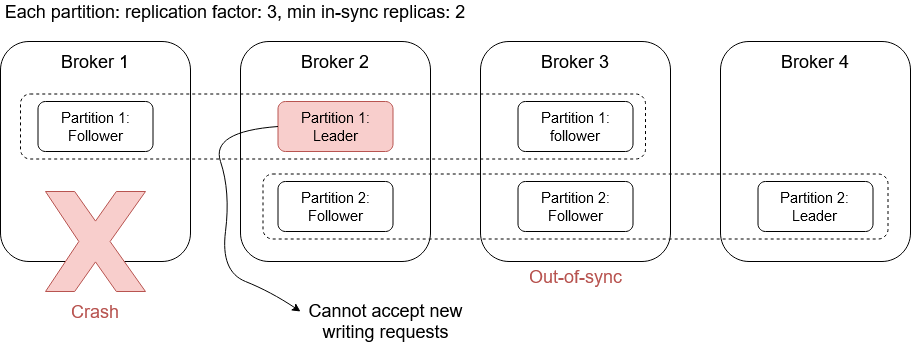
\includegraphics[width=\linewidth]{images/broker-failover-kafka.png}
	\caption{Availability on Kafka cannot be guaranteed when partition is under-replicated.}
	\label{fig:brokerfailoverkafka}
\end{figure}
In figure \ref{fig:brokerfailoverkafka}, when broker 1 fails and the replica of partition 1 on broker 3 becomes out-of-sync with the leader, broker 2 cannot accept new writing requests for partition 1 since it cannot meet the minimum in-sync replicas of two. Broker 4 cannot support to ensure the availability since it does not retain the copy of partition 1. In this case, the availability is compromised for the reliability of data persistence.

If all in-sync replicas including the leader fail at the same time, the remaining replicas of the partition are all lagged behind without having the latest committed messages. In this case, users can choose between availability and consistency of data \cite{kafkadatareplication}. Users can either allow one out-of-sync replica to become the new leader to not disrupt the requests handling and risk losing some records or wait until one in-sync replica goes back online and reject all requests to the failed partition in the meantime. 

Since a Kafka broker also serves the persistence of records, there is a trade-off between its availability and consistency of data. The failover mechanism of Kafka give users the flexibility to manage this trade-off.

\large \textbf{Apache Pulsar}\\
\normalsize
\textbf{Scalability of storage and computing server}\\
In a Pulsar cluster, the cluster of Pulsar brokers is in charge of handling requests from clients while the Bookkeeper cluster is used for data storage. There two layers of processing and storage can be scaled independently.

On the requests-serving layer, each topic is owned by only one broker in the cluster and all requests to this topic will be directed to this broker only. When a new topic is created, the load manager in the Pulsar cluster assigns it to the broker with the least load. Moreover, whenever a broker is overloaded or goes down, the load manager also automatically triggers the balancing to distribute the topics to other brokers \cite{pulsarloadbalance}. As a result, scaling the cluster of brokers is very straightforward. 

On the storage layer, scalability is achieved by the built-in mechanism of Bookkeeper. As elaborated in section \ref{section:eventstorage}, messages are replicated on Bookkeeper cluster in fragments. Each fragment has a different ensemble which is determined by the Pulsar broker. When a new Bookkeeper nodes is started, they will automatically be considered when choosing the ensemble for the next fragment and can start to share the load with other existing nodes. 
\begin{figure}[h]
	\centering
	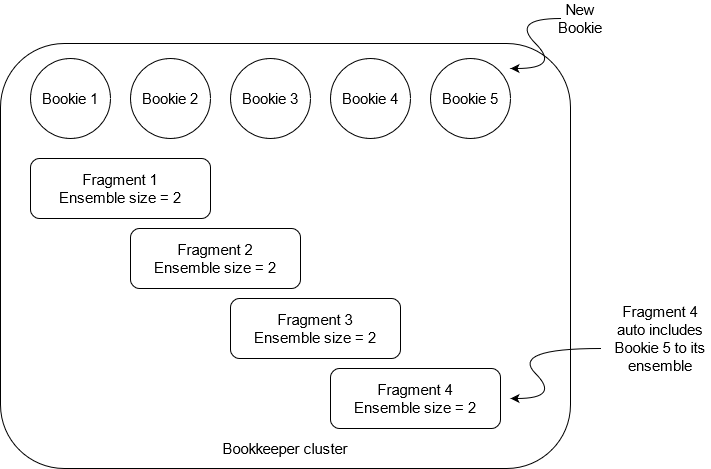
\includegraphics[width=\linewidth]{images/scalability-pulsar.png}
	\caption{Storage layer of Pulsar can be scaled up seamlessly by starting new Bookkeeper instances.}
	\label{fig:scalabilitypulsar}
\end{figure}

If a Bookkeeper node is shut down, some fragments with messages persisted on this node will be under-replicated. However, the auto recovery feature of Bookkeeper can detect this and re-replicate these messages to other running nodes to maintain the replication quorum \cite{bookkeeperadmin}.
\newpage
\textbf{Broker failover mechanism}\\
The brokers are registered to the Zookeeper and regularly kept track of its online status. When a broker is detected to be failed by Zookeeper, its topic will be assigned to other online brokers in the cluster. Apache Pulsar uses the fencing mechanism of BookKeeper to prevent the disconnected broker from writing new message to the topic \cite{bookkeeperprotocol}. This ensures that at any time, only one broker can serve writing requests to a topic.

Because the processing and persisting layers of Pulsar are completely separated, the failover mechanism does not have to consider the reliability of data persistence as in Kafka. As long as there is an online broker, new requests can continue to be accepted. If the requests are handled successfully, clients will receive confirmations from broker and be ensured about the reliability of data. 

\large \textbf{NATS Streaming}\\
\normalsize
\textbf{Scalability of storage and computing server}\\
In both operational modes of NATS Streaming cluster, namely clustering and fault-tolerance, only one server in the cluster can handle read and write requests from clients \cite{natsstreaming}. To support horizontal scaling of requests-serving layer, NATS Streaming provides the partitioning feature \cite{natspartitioning}. This feature is not compatible with clustering mode. With this feature, the normal fault tolerant cluster can be partitioned into a number of smaller sub-clusters, each of which is independently in charge of handling requests for a subset of channels and has a separated datastore to persist messages of these channels. 

Each sub-cluster must be strictly configured with a fixed set of channels. Requests to different channels will be balanced among the server instances in the cluster. New sub-cluster can always be added to the cluster to handle more channels. 
%To save resources with the partitioning feature, active server instance of a sub-cluster can run along with standby instances of other sub-clusters on one host machine. This would not have a significant impact on the performance because the standby instances only forward requests and do not use much resource. 
\begin{figure}[h]
	\centering
	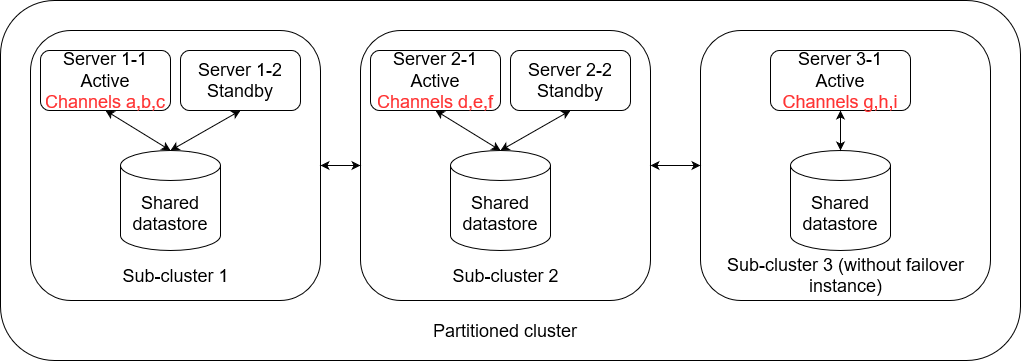
\includegraphics[width=\linewidth]{images/scalability-nats.png}
	\caption{Request-serving layer of NATS Streaming can be horizontally scaled with the partitioning feature.}
	\label{fig:scalabilitynats}
\end{figure}

Nevertheless, this scaling mechanism has many limitations. Firstly, this feature cannot be used together with clustering mode. Therefore, it cannot use the data replication feature provided by NATS Streaming. The set of assigned channels for each sub-cluster cannot be changed in runtime. If new channels are required, the sub-cluster must be stopped for reconfiguration. Moreover, because each sub-cluster has a completely separated storage location for all assigned channel, it is not possible to dynamically transfer the ownership of some channels on one sub-cluster to another for load balancing.
 
On the storage layer, the scalability depends on the chosen pluggable data store. For instance, if \emph{file} store is chosen as the persistence layer, a scalable network filesystem can always be used. When \emph{SQL} store is used, the scalability is governed by the relational database technology. However, this relies entirely on the setup of users without any supported feature from NATS Streaming. 

In short, scalability on NATS Streaming is possible for both storage and requests-serving layers. However, most of the configurations and administration tasks are not covered by NATS but instead must be handled manually by users. 

\textbf{Broker failover mechanism}\\
In the clustering mode, the servers in the cluster coordinate with each other using RAFT consensus algorithm \cite{raftalg}. Only the one elected leader in the cluster can serve requests from clients. In case the leader fails, one of the followers will be elected as the new leader. This mode is resilient to split-brain since the Raft algorithm uses majority vote for both leader election and acknowledgement of writing requests. However, if more than half of the servers in the cluster fails, there will be not enough nodes for leader election in case of failure. In this case, the cluster cannot accept new request even when there are still online servers. The availability is automatically compromised for data consistency. 

In the fault-tolerance mode, several server instances are attached to a share datastore \cite{natsstreaming}. At any time, only one active node holds the exclusive lock on the datastore to serve requests. If the active node fails, all standby instances will try to obtain the lock on the data storage and the first to be successful will become the new active node. This failover mechanism requires less overhead as in the clustering mode since no leader re-election is required. In this mode, as long as there is an online server, new requests can be accepted.